\chapter{Beobachtungen, Dunkle Materie und der kosmologische Fit}

\lectureoverview{Beobachtungen erhalten erst dann eine Bedeutung, wenn sie mit einem kosmologischen Modell verknüpft werden. Wir beginnen mit der Friedmann-Gleichung und den drei homogenen räumlichen Geometrien, gliedern die heutige kosmische Energiebilanz in Strahlung, Materie, Vakuumenergie und Krümmung und rekonstruieren, warum ein offenes Universum einst unvermeidlich schien. Die Rotationskurven von Galaxien machen dann die fehlende gravitierende Materie sichtbar und führen zur Dynamik eines kalten, schwach wechselwirkenden Halos. Schließlich machen Rotverschiebung, Helligkeit und Quellenzahlen aus einem probeweise angenommenen Expansionsverlauf beobachtbare Kurven. Das alte Modell aus Materie und Krümmung scheitert; ein Materieanteil von etwa \(0.3\), ein Vakuumenergieanteil von etwa \(0.7\) und eine sehr geringe Krümmung ergeben den erfolgreichen Fit dieser Vorlesung.}

\section{Die Beobachtungen wieder in die Gleichungen einsetzen}

Astronomische Tatsachen lassen sich nicht isoliert interpretieren. Zunächst brauchen wir die Gleichungen, die angeben, welche Kombinationen von Beobachtungen ein Universum von einem anderen unterscheiden. Für ein homogenes und isotropes Universum ist die Friedmann-Gleichung der Ausgangspunkt,
\begin{equation}
\left(\frac{\dot a}{a}\right)^2
=
\frac{8\pi G}{3}\rho-\frac{k}{a^2}.
\label{eq:c06-friedmann}
\end{equation}
Die Größe
\begin{equation}
H(t)=\frac{\dot a(t)}{a(t)}
\label{eq:c06-hubble}
\end{equation}
ist die Hubble\emph{funktion}. Ihr heutiger Wert \(H_0\) wird üblicherweise Hubble-Konstante genannt, doch \(H(t)\) ist im Laufe der kosmischen Geschichte nicht konstant. Wenn Astronomen einen Wert in Kilometern pro Sekunde und Megaparsec angeben, geben sie \(H_0\) an.

Der normierte Krümmungsparameter kann nur drei Werte annehmen,
\begin{equation}
k\in\{+1,0,-1\},
\end{equation}
die jeweils einer sphärischen, flachen und hyperbolischen räumlichen Geometrie entsprechen. Die übliche FRW-Metrik lässt sich schreiben als
\begin{equation}
ds^2=-dt^2+a(t)^2\left[dr^2+\xi(r)^2d\Omega_2^2\right],
\label{eq:c06-frw}
\end{equation}
wobei
\begin{equation}
\xi(r)=
\begin{cases}
\sin r, & k=+1,\\
r, & k=0,\\
\sinh r, & k=-1.
\end{cases}
\label{eq:c06-xi}
\end{equation}
Diese Notation erfüllt zwei Zwecke. Sie fasst die drei Geometrien in einer Metrik zusammen und liefert später die Fläche einer Kugel und damit die Anzahl der Quellen in einer radialen Schale. Die Wahl von \(k\) und eine Gleichung für \(a(t)\) ergeben somit bereits ein Modell mit beobachtbaren Konsequenzen.

\section{Die heutige kosmische Energiebilanz}

Die Energiedichte hat im hier betrachteten Modell drei Hauptkomponenten: Strahlung, nichtrelativistische Materie und Vakuumenergie. Nimmt man die Krümmung in dieselbe Bilanz auf, erhält man
\begin{equation}
\frac{C_r}{a^4}
+\frac{C_m}{a^3}
+\Lambda
-\frac{k}{a^2}
=H^2.
\label{eq:c06-budget}
\end{equation}
Hier verwendet \(\Lambda\) die Normierung aus der vorangegangenen Vorlesung, \(\Lambda=(8\pi G/3)\rho_{\rm vac}\). Die Strahlungsdichte nimmt wie \(a^{-4}\) ab, die Materiedichte wie \(a^{-3}\); die Vakuumenergie wird nicht verdünnt, und die Krümmung skaliert wie \(a^{-2}\). Krümmung ist keine materielle Energiedichte, doch ihre Aufnahme neben den anderen Termen macht die heutige Nebenbedingung deutlich: Die vier Beiträge müssen zusammen \(H_0^2\) ergeben.

Definieren wir ihre heutigen Anteile durch
\begin{equation}
\begin{aligned}
\Omega_r&=\frac{C_r/a_0^4}{H_0^2},
&\qquad
\Omega_m&=\frac{C_m/a_0^3}{H_0^2},\\
\Omega_\Lambda&=\frac{\Lambda}{H_0^2},
&
\Omega_k&=\frac{-k/a_0^2}{H_0^2}.
\end{aligned}
\label{eq:c06-omegas}
\end{equation}
Dann gilt
\begin{equation}
\boxed{\Omega_r+\Omega_m+\Omega_\Lambda+\Omega_k=1.}
\label{eq:c06-sum-rule}
\end{equation}
Die \(\Omega\) sind heute ausgewertete Verhältnisse, keine zeitlich konstanten Größen. Beachten Sie außerdem die Vorzeichenkonvention: \(k=-1\) ergibt ein positives \(\Omega_k\).

\subsection{Wie die ersten Beiträge gemessen werden}

Hubble bestimmte die lokale Expansionsrate, indem er die Rotverschiebung durch die Rezessionsbewegung mit der Entfernung verglich. Bei kleinen \(z\) liefert die Rotverschiebung die Geschwindigkeit; eine kalibrierte Helligkeit liefert die Entfernung. Sein erster Zahlenwert war erheblich falsch, aber die Methode war richtig. Da die Galaxien vergleichsweise nahe waren, erfasste die Messung nur einen kleinen Teil der kosmischen Geschichte; \(H\) konnte daher als heutiger Wert behandelt werden.

\begin{classroomqa}
\audiencequestion{Wie kann man aus der Helligkeit auf die Entfernung schließen, wenn die intrinsische Helligkeit nicht schon bekannt ist?}
\lecturerresponse{Das geht nicht in einem Schritt. Die kosmische Entfernungsleiter beginnt mit der Parallaxe naher Sterne. Cepheiden in diesem kalibrierten Bereich zeigen eine Perioden-Leuchtkraft-Beziehung und dienen als Standardkerzen für größere Entfernungen. Überlappende Kalibrierungen führen die Leiter weiter hinaus; für die später betrachteten kosmologischen Rotverschiebungen sind Supernovae die besten Standardkerzen. Die Entfernung wird also aus einer Kette von Standards erschlossen und nicht aus der willkürlichen Annahme, alle Objekte leuchteten gleich hell. \lecturetimestamp{00:10:00--00:11:32}}
\end{classroomqa}

\begin{classroomqa}
\audiencequestion{Sind \(C_r\) und \(C_m\) Konstanten, obwohl sich ihre Dichten ändern?}
\lecturerresponse{Ja. Die Koeffizienten bleiben fest, während die Faktoren \(a^{-4}\) und \(a^{-3}\) die Zeitabhängigkeit tragen. Die Vakuumenergie ist konstant, und die Krümmung skaliert wie \(a^{-2}\). Gerade wegen dieser unterschiedlichen Potenzen ändern sich die relativen Beiträge von einer kosmischen Epoche zur nächsten. \lecturetimestamp{00:11:35--00:12:02}}
\end{classroomqa}

Der Strahlungsbeitrag lässt sich lokal anhand des Photonenhintergrunds messen. Der größte Teil davon ist die kosmische Mikrowellenhintergrundstrahlung, und ihre heutige Energiedichte ist im Vergleich zu den anderen wichtigen Komponenten sehr klein. Man benötigt ein ausreichend großes Mittelungsvolumen, muss aber nicht weit entlang des vergangenen Lichtkegels zurückblicken, um festzustellen, dass \(\Omega_r\) heute vernachlässigbar ist.

Die sichtbare Materie wird anhand von Galaxien, Sternpopulationen, Wasserstoff und interstellarem Gas abgeschätzt. Die Methoden sind technisch, aber konzeptionell nicht undurchsichtig: Man bestimmt den typischen Stern- und Gasgehalt, summiert ihn über die Galaxien und mittelt über ein großes Volumen. In der Vorlesung wird als grobe historische Größenordnung eine Protonenmasse pro Kubikmeter angegeben. Das ist deutlich mehr als die Strahlungsdichte, aber immer noch bemerkenswert wenig.

\begin{classroomqa}
\audiencequestion{Wie wird Dunkle Materie in dieser Bilanz berücksichtigt?}
\lecturerresponse{Darauf kommen wir noch; zunächst rekonstruieren wir bewusst die ältere Schlussfolgerung, die allein auf leuchtender Materie beruhte. Die historische Reihenfolge ist wichtig: Sie zeigt genau, welche scheinbare Schlussfolgerung durch Dunkle Materie korrigiert wurde und welche Lücke dadurch nicht geschlossen wurde. \lecturetimestamp{00:15:08--00:15:40}}
\end{classroomqa}

\section{Warum ein offenes Universum einst notwendig schien}

Im älteren Bild wurde die Strahlung zu Recht als vernachlässigbar eingestuft, die Vakuumenergie gleich null gesetzt und unter Materie nur das durch elektromagnetische Strahlung sichtbare Material verstanden. Die daraus folgende Abschätzung lautete ungefähr
\begin{equation}
\Omega_r\simeq0,
\qquad
\Omega_\Lambda=0,
\qquad
\Omega_m^{\rm luminous}\sim\frac{1}{20}\text{--}\frac{1}{30}.
\end{equation}
Die Summenregel schien dann zu erzwingen,
\begin{equation}
\Omega_k\simeq1.
\end{equation}
Da ein positiver Krümmungsbeitrag \(-k/a_0^2>0\) bedeutet, folgte daraus \(k=-1\): ein offenes Universum mit negativer Krümmung. Diese Zahlen rekonstruieren das ältere Argument; sie sind keine moderne Parameterschätzung.

Um die Krümmungsskala zu interpretieren, kehren wir zur Lösung für ein materiedominiertes Universum zurück:
\begin{equation}
a(t)\propto t^{2/3}.
\end{equation}
Ableiten und anschließendes Dividieren durch \(a\) ergibt
\begin{equation}
H(t)=\frac{\dot a}{a}=\frac{2}{3t}.
\label{eq:c06-matter-h}
\end{equation}
Für das heutige Alter \(T\) gilt
\begin{equation}
H_0\simeq\frac{2}{3T}.
\end{equation}
Die Hubble-Zeit liegt also in derselben Größenordnung wie das Alter des Universums. Der Vergleich mit strahlungsdominierter Expansion,
\begin{equation}
a(t)\propto t^{1/2},
\qquad
H(t)=\frac{1}{2t},
\end{equation}
zeigt, dass diese umgekehrte Proportionalität zum Alter nicht spezifisch für Staub ist.

\begin{figure}[htbp]
\centering
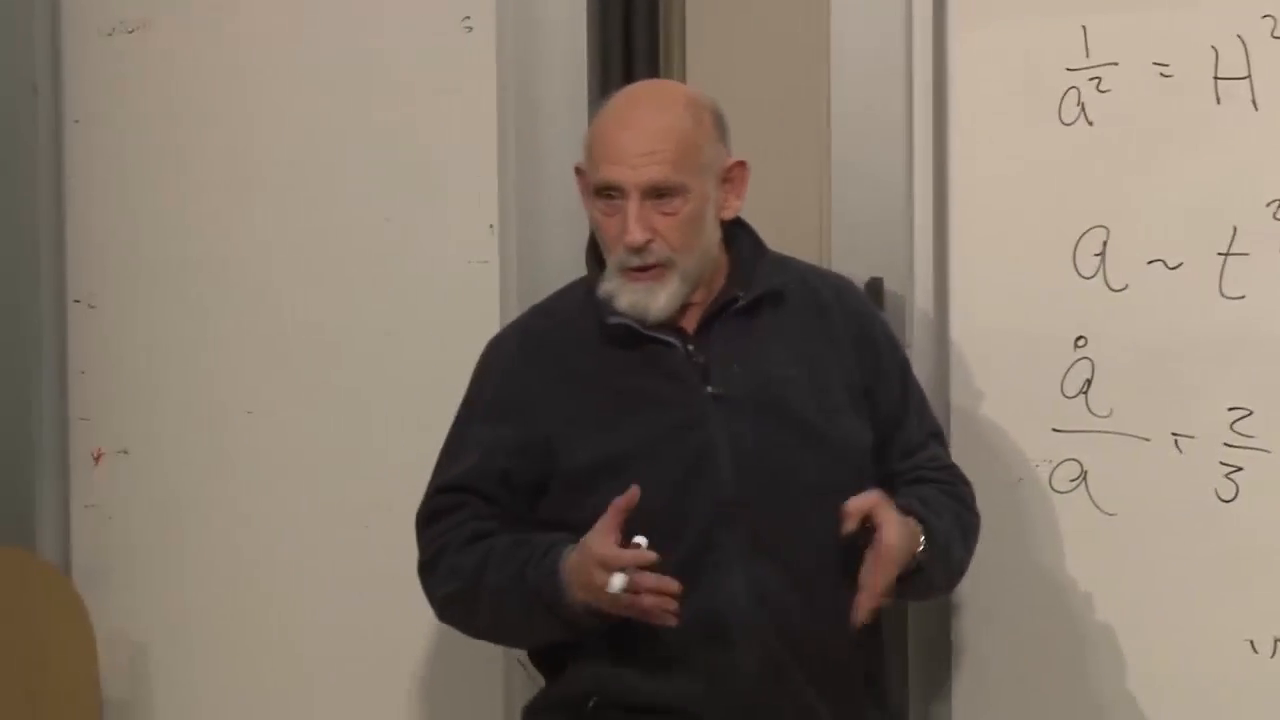
\includegraphics[width=0.72\textwidth]{lecture_06_figure_02.png}
\caption{Tafelbild zur Epoche der Materiedominanz. Sichtbar sind die Einträge \(a\sim t^{2/3}\) und \(\dot a/a=2/(3t)\); der Dozent verdeckt den übrigen Teil der Tafel, daher wird dem Bild keine weitere Gleichung zugeschrieben.}
\label{fig:c06-age-board}
\lectureframe{00:24:41.615}
\end{figure}

\begin{classroomqa}
\audiencequestion{Welche Einheiten hat die Hubble-Konstante, und wo steckt die Lichtgeschwindigkeit?}
\lecturerresponse{Da \(H\) Geschwindigkeit und Entfernung miteinander verknüpft, hat es die Einheit einer inversen Zeit. Man kann es in inversen Sekunden oder Jahren angeben oder in der für Astronomen üblichen äquivalenten Einheit Kilometer pro Sekunde und Megaparsec. Für die Beziehung \(H\sim1/T\) ist kein zusätzlicher Faktor \(c\) erforderlich. Ein Faktor \(c\) tritt nur auf, wenn die Zeit \(T\) in eine Länge wie \(cT\) umgerechnet wird. \lecturetimestamp{00:22:50--00:24:25}}
\end{classroomqa}

Hubbles ursprünglicher Wert \(H_0\) war ungefähr um eine Größenordnung zu groß, sodass das entsprechende Hubble-Alter zu kurz ausfiel: In der gerundeten Gegenüberstellung der Vorlesung lag es bei etwa einer Milliarde statt zehn Milliarden Jahren. Eine bessere Kalibrierung korrigierte den Zahlenwert, ohne die Logik zu ändern, nach der \(H_0^{-1}\) eine kosmische Zeitskala ist.

Die alte Schlussfolgerung zur Krümmung lautet nun
\begin{equation}
\frac{1}{a_0^2}\sim H_0^2\sim\frac{1}{T^2}.
\end{equation}
In Einheiten mit \(c=1\) wurde der Krümmungsradius \(a_0\) daher auf eine Größenordnung des Alters \(T\) geschätzt; mit wieder eingesetzten gewöhnlichen Einheiten entsprach das einer Größenordnung von \(cT\). Die Vorlesung nimmt diese Aussage unmittelbar als Beschreibung des wirklichen Universums zurück. Sie gibt die Schlussfolgerung wieder, zu der man mehrere Jahrzehnte zuvor gelangte, nachdem man die damals für vernachlässigbar gehaltenen Terme weggelassen hatte.

\begin{classroomqa}
\audiencequestion{Wenn die Krümmung heute dominieren sollte, warum verwendet man dann das Materiedominanzgesetz \(a\propto t^{2/3}\)?}
\lecturerresponse{Weil die Materie wie \(a^{-3}\) skaliert, während die Krümmung nur wie \(a^{-2}\) skaliert. Bei kleinerem \(a\) überwiegt die Materie. Die Krümmung konnte erst spät wichtig werden; daher beschrieb die Materiedominanz den größten Teil der verstrichenen Zeit weiterhin gut und hielt \(H_0\) in der Größenordnung von \(1/T\). Eine vollständige Lösung für ein Gemisch würde den Zahlenfaktor korrigieren, nicht aber das Argument zur Zeitskala entkräften. \lecturetimestamp{00:49:20--00:50:17}}
\end{classroomqa}

\section{Dunkle Materie aus der Galaxiendynamik}

Es gibt zwei praktische Wege, Materie zu erfassen. Der eine zählt Material, das Licht aussendet oder absorbiert. Der andere erschließt Masse aus der Gravitation. Oort fand in den frühen 1930ern eine anomale Galaxiendynamik, und Zwicky entdeckte eine entsprechende Massendifferenz in Galaxienhaufen. Die Befunde zeigten, dass die gravitierende Materie die leuchtende Materie übertraf. Gewöhnliche geladene Materie strahlt und stößt zusammen; die fehlende Komponente war zunächst durch ihre Gravitationswirkung bekannt.

\begin{classroomqa}
\audiencequestion{Zählen diffuse Gase und zentrale Schwarze Löcher zur leuchtenden Materie?}
\lecturerresponse{Diffuses Gas wird berücksichtigt, soweit sich seine Menge aus seinem elektromagnetischen Verhalten erschließen lässt. Ein zentrales supermassereiches Schwarzes Loch kann in die bekannte Massenbilanz eingehen, macht aber nur einen kleinen Teil der Gesamtmasse einer Galaxie aus und ist im Zentrum konzentriert. Es kann keine Diskrepanz erklären, die weit außerhalb des leuchtenden Zentrums fortbesteht. \lecturetimestamp{00:29:50--00:31:14}}
\end{classroomqa}

Betrachten wir einen Stern, der sich näherungsweise auf einer Kreisbahn mit Radius \(r\) bewegt. Wäre nahezu die gesamte Masse \(M\) nahe dem galaktischen Zentrum konzentriert, ergäbe das Newtonsche Gesetz
\begin{equation}
\frac{GM}{r^2}=\frac{v^2}{r},
\end{equation}
und damit
\begin{equation}
v^2=\frac{GM}{r},
\qquad
v(r)\propto r^{-1/2}.
\label{eq:c06-kepler}
\end{equation}
Dies ist der außerhalb einer zentralen Massenverteilung erwartete Kepler-Abfall.

\begin{figure}[htbp]
\centering
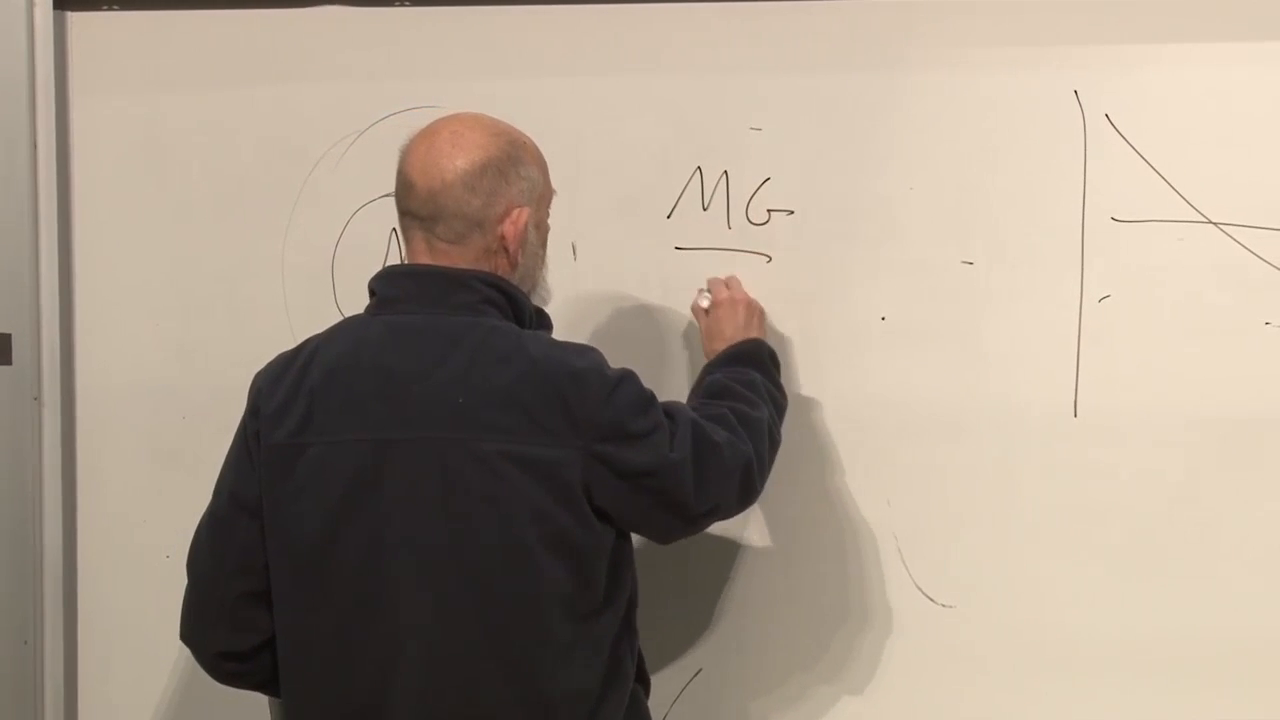
\includegraphics[width=0.78\textwidth]{lecture_06_figure_03.png}
\caption{Tafelbild zu Rotationskurven beim Übergang von einer zentralen Masse zur eingeschlossenen Masse \(M(r)\). Sichtbar sind nur \(MG\), der Bruchstrich, die Bahnskizze und Teile der Kurvenskizzen; Gleichung~\eqref{eq:c06-kepler} stammt aus der mündlichen Herleitung.}
\label{fig:c06-rotation-board}
\lectureframe{00:34:53.642}
\end{figure}

\begin{figure}[htbp]
\centering
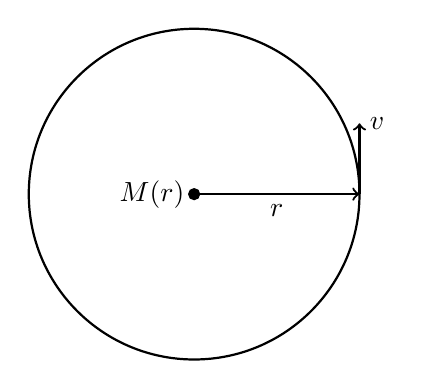
\begin{tikzpicture}[scale=1.0]
\filldraw (0,0) circle (2pt) node[left] {\(M(r)\)};
\draw[thick] (0,0) circle (2.1);
\draw[->,thick] (0,0)--(2.1,0) node[midway,below] {\(r\)};
\draw[->,thick] (2.1,0)--(2.1,0.9) node[right] {\(v\)};
\end{tikzpicture}
\caption{Konstruktion einer Kreisbahn, mit der sich aus einer gemessenen Umlaufgeschwindigkeit die eingeschlossene Masse erschließen lässt.}
\label{fig:c06-orbit-redraw}
\end{figure}

Beobachtete galaktische Rotationskurven fallen nicht auf diese Weise ab; über einen beträchtlichen Radialbereich sind sie annähernd flach. Ersetzen wir die feste zentrale Masse durch die eingeschlossene Masse \(M(r)\):
\begin{equation}
\frac{G M(r)}{r^2}=\frac{v(r)^2}{r}.
\end{equation}
Ist \(v(r)\) annähernd konstant, so gilt
\begin{equation}
\boxed{M(r)\propto r.}
\label{eq:c06-enclosed-mass}
\end{equation}
Gemeint ist die Gesamtmasse innerhalb des Radius \(r\), nicht die lokale Dichte. Die gravitierende Masse nimmt weit über den Bereich hinaus weiter zu, in dem sich der größte Teil des Sternenlichts konzentriert. Bewegungen senkrecht zu den galaktischen Scheiben weisen außerdem auf eine annähernd kugelförmige Verteilung hin: einen dunklen Halo statt einer zweiten dünnen Scheibe.

\begin{classroomqa}
\audiencequestion{Gibt es eine einfache Theorie, die erklärt, warum die Rotationskurve so flach ist?}
\lecturerresponse{Nicht im Rahmen dieses Arguments. Simulationen der Galaxienentstehung können solche Profile als natürlich erscheinen lassen, aber die Vorlesung beansprucht keine kurze Herleitung. Die gesicherte Aussage ist eine Beobachtung: Ein annähernd konstantes \(v\) bedeutet, dass die eingeschlossene Masse ungefähr linear zunimmt. Die Eleganz dieser Beziehung sollte nicht mit einer einfachen Erklärung der Galaxienentstehung verwechselt werden. \lecturetimestamp{00:35:58--00:37:33}}
\end{classroomqa}

\begin{classroomqa}
\audiencequestion{Sind Spiralarmmuster einfach materielle Windräder, die durch die veränderliche Winkelgeschwindigkeit \(v/r\) entstehen?}
\lecturerresponse{Ein einfaches Windradbild funktioniert nicht. Das sichtbare Muster muss sich nicht gemeinsam mit den einzelnen Sternen drehen; Dichtewellen oder Wellen der Sternentstehung sind mögliche Beschreibungen. Die Vorlesung nutzt diese Unsicherheit, um die robuste Schlussfolgerung zum Halo von dem komplizierteren Problem der Spiralstruktur abzugrenzen. \lecturetimestamp{00:37:35--00:38:34; 00:47:03--00:47:47}}
\end{classroomqa}

Die erschlossene Dunkle Materie hat eine Masse, die um ein Mehrfaches größer ist als die leuchtende Masse; in der Vorlesung wird dafür lediglich eine grobe Größenordnung zwischen fünf und zehn angegeben. Der Halo reicht außerdem über die sichtbare Galaxie hinaus. Dies sind bewusst grobe historische Größenordnungen, keine präzisen, für jedes System geltenden Verhältnisse.

\section{Welche Eigenschaften Dunkle Materie haben muss}

Warum bildet gewöhnliche Materie helle, kompakte Scheiben, während Dunkle Materie in einem ausgedehnten Halo bleibt? Leuchtende Materie kann durch elektromagnetische Stöße und Strahlung mechanische Energie verlieren. Wenn sie Energie abgibt, kann die Gravitation sie in eine dichtere Konfiguration ziehen. Dunkle Materie scheint elektrisch neutral zu sein und viel schwächer zu wechselwirken. Ihre Teilchen umlaufen den Halo nahezu ohne Stöße oder Strahlung und verlieren daher selbst über Milliarden Jahre nicht genug Energie, um sich in der leuchtenden Scheibe anzusammeln. Gravitationsstrahlung infolge galaktischer Bewegung ist viel zu schwach, um als alternativer Abkühlungsmechanismus zu dienen.

\begin{classroomqa}
\audiencequestion{Bedeutet schwache Wechselwirkung, dass Dunkle Materie einem anderen Gravitationsgesetz folgt?}
\lecturerresponse{Nein. Es wird angenommen, dass sie auf gewöhnliche Weise gravitativ wechselwirkt. Schwache Wechselwirkung bedeutet hier, dass nichtgravitative Stöße und elektromagnetische Strahlung fehlen oder stark unterdrückt sind. Zwei dunkle Teilchen ziehen einander weiterhin gravitativ an; diese Anziehung strukturiert einen Halo, führt aber nicht zu einer effizienten Abgabe orbitaler Energie. \lecturetimestamp{00:42:36--00:43:35}}
\end{classroomqa}

\begin{classroomqa}
\audiencequestion{Welche Beobachtungen zeigen, dass dies keine Besonderheit einer einzelnen galaktischen Rotationskurve ist?}
\lecturerresponse{Die Hinweise treten auf verschiedenen Skalen auf: bei der Bewegung von Sternen innerhalb von Galaxien, bei Bewegungen senkrecht zu galaktischen Ebenen, bei Wechselwirkungen zwischen Galaxien und in der Dynamik ganzer Galaxienhaufen. Die Beispiele von Oort und Zwicky waren verschiedene Ausprägungen desselben Problems fehlender Gravitation. \lecturetimestamp{00:42:00--00:42:36}}
\end{classroomqa}

\begin{classroomqa}
\audiencequestion{Sollte sich Dunkle Materie um Schwarze Löcher und galaktische Zentren ansammeln?}
\lecturerresponse{Ihre Dichte nimmt zu einem Gravitationszentrum hin tatsächlich zu. Die historische Abfolge verlief jedoch wahrscheinlich umgekehrt zu einem Halo, der sich um ein bereits vorhandenes Schwarzes Loch bildet. Dunkle Halos bildeten große Gravitationsmulden; baryonische Materie fiel anschließend hinein und bildete Galaxien, Sterne und zentrale Schwarze Löcher. Das Schwarze Loch macht nur einen kleinen Teil der Masse aus. Bei der Suche nach Annihilationsprodukten richtet man den Blick dennoch zum galaktischen Zentrum, weil dort eine höhere Dichte Dunkler Materie erwartet wird. \lecturetimestamp{00:43:36--00:45:43}}
\end{classroomqa}

\begin{classroomqa}
\audiencequestion{Ist Dunkle Materie ein Gas, Staub, kompakte Klumpen oder einzelne Teilchen? Könnte ein Teil davon in Sonnennähe gebunden sein?}
\lecturerresponse{Ihre mikroskopische Natur ist unbekannt. Gewöhnlicher Staub wird jedoch durch elektromagnetische Kräfte gebunden, also gerade durch Wechselwirkungen, die Dunkler Materie offenbar fehlen. Daher geht man standardmäßig von einer verdünnten Population einzelner Teilchen aus. Einige davon könnten sich gravitativ in Sonnennähe konzentrieren; ihre Dichte ist aber viel zu gering, um mit der Sonnenanziehungskraft zu konkurrieren oder die Planetendynamik zu stören. \lecturetimestamp{00:45:43--00:47:02; 00:58:41--00:59:29}}
\end{classroomqa}

Die zweite zentrale Voraussetzung ist, dass Dunkle Materie verklumpt. Eine heiße Population mit relativistischen Zufallsgeschwindigkeiten widersteht der gravitativen Aggregation; eine kalte Population kann in Potenzialmulden fallen. Gewöhnliche leichte Neutrinos hätten sich als heiße Dunkle Materie verhalten und liefern nicht die erforderliche Hauptkomponente der Galaxien. In diesem Zusammenhang bedeutet \emph{kalt}nichtrelativistisch im lokalen kosmologischen Bezugssystem und nicht, dass die Temperatur im Labor buchstäblich null beträgt.

\begin{classroomqa}
\audiencequestion{Ergibt sich aus der Forderung nach kalter, verklumpender Dunkler Materie ein Massenbereich?}
\lecturerresponse{Das hängt von der Quantenstatistik und der Entstehungsgeschichte ab. Sehr leichte Fermionen können nicht alle denselben langsamen Zustand besetzen und unterliegen starken Einschränkungen. Sehr leichte Bosonen können einen kohärenten Bose-kondensierten Zustand einnehmen; Axionen sind das Beispiel der Vorlesung. Alternativ können schwerere, schwach wechselwirkende Teilchen auch ohne Kondensation kalt sein. Aus diesem Argument folgt daher keine einzelne, modellunabhängige Massengrenze. \lecturetimestamp{00:53:17--00:54:52; 00:56:42--00:58:05}}
\end{classroomqa}

\begin{classroomqa}
\audiencequestion{Hätten Beschleuniger die Teilchen nicht längst finden müssen?}
\lecturerresponse{Nur unter zusätzlichen Annahmen. Haben die Teilchen ungefähr typische Wirkungsquerschnitte der schwachen Wechselwirkung und Massen innerhalb der Reichweite von Beschleunigern, könnte ihre Erzeugung in Kollidern möglich sein. Die Erwartung der Vorlesung, bald neue Erkenntnisse zu gewinnen, war ausdrücklich spekulativ und an ihre Zeit gebunden. Ein Teilchen könnte aber auch zu schwer sein oder zu schwach wechselwirken, um mit den verfügbaren Experimenten nachweisbar zu sein. \lecturetimestamp{00:54:52--00:55:54}}
\end{classroomqa}

\begin{classroomqa}
\audiencequestion{Könnte Dunkle Materie einfach in einer unbeobachteten zusätzlichen Dimension existieren?}
\lecturerresponse{Ein solcher Mechanismus ist für diese Diskussion nicht erforderlich. Dunkle Materie wird bereits gravitativ beobachtet und könnte schlicht aus ungewöhnlichen Teilchen bestehen, die nahezu gar nicht mit gewöhnlicher Materie wechselwirken. Eine schwache Wechselwirkung bedeutet nicht, dass die Teilchen außerhalb der beobachtbaren Raumzeit liegen. \lecturetimestamp{00:55:54--00:56:41}}
\end{classroomqa}

Die Abänderung der Gravitation statt der Ergänzung um unbeobachtete Materie ist eine logische Alternative. Nach Einschätzung der Vorlesung erklärte damals keine ebenso einfache Modifikation die Befunde auf allen relevanten Skalen und bewahrte zugleich die erfolgreichen Gesetze des Sonnensystems. Daher wird die Teilcheninterpretation bevorzugt; ihre mikrophysikalische Natur bleibt jedoch unbekannt.

\section{Dunkle Materie schließt die alte Bilanzlücke nicht}

Dunkle Materie vergrößert den Materiebeitrag um ein Mehrfaches, doch die alte Diskrepanz zwischen leuchtender Materie und \(H_0^2\) lag ungefähr beim Faktor fünfundzwanzig. Die Lücke wird dadurch kleiner, aber \begin{equation}
\frac{C_m}{a_0^3}=H_0^2.
\end{equation} gilt weiterhin nicht. Im alten Modell ohne \(\Lambda\) war nach wie vor ein positiver Krümmungsbeitrag zur Energiebilanz und damit \(k<0\) erforderlich. Ein solches offenes Modell war logisch widerspruchsfrei; entscheidend ist, dass Dunkle Materie allein die moderne Antwort nicht ergab.

\begin{classroomqa}
\audiencequestion{Was hielten Kosmologen vor dem modernen Fit tatsächlich von der Krümmung?}
\lecturerresponse{Die Befundlage war verwirrend, und die vorherige Präferenz für ein geschlossenes, begrenztes Universum stand bisweilen im Widerspruch zur Materiebilanz. Sobald die alten Annahmen widerspruchsfrei zusammengeführt wurden, war negative Krümmung die naheliegende Schlussfolgerung. Dieser historische Konsens blieb vorläufig, da weder Dunkle Materie noch Vakuumenergie so sicher berücksichtigt wurden, wie es heute der Fall ist. \lecturetimestamp{00:50:17--00:51:50}}
\end{classroomqa}

Wir müssen das Modell also prüfen, statt seine Gültigkeit aus einer einzigen Bilanzgleichung abzuleiten. Ein Modell besteht aus einer Krümmungswahl \(k\) und einem Expansionsverlauf \(a(t)\), beziehungsweise aus einer Menge von Zustandsgleichungen der Materie und heutigen Parametern, aus denen \(a(t)\) berechnet wird. Das alte Modell enthält Materie und negative Krümmung, vernachlässigbare Strahlung und keine kosmologische Konstante.

\section{Geometrie in Beobachtbares überführen}

\subsection{Quellenzahlen und Helligkeit bei eingefrorener Geometrie}

Vernachlässigen wir vorübergehend die kosmische Entwicklung. In einem homogenen Universum ist die Anzahl der Quellen in einer komovierenden Schale proportional zu ihrer Fläche:
\begin{equation}
dN\propto \xi(r)^2\,dr.
\label{eq:c06-shell-count}
\end{equation}
Also gilt
\begin{equation}
dN\propto
\begin{cases}
\sin^2r\,dr, & k=+1,\\
r^2\,dr, & k=0,\\
\sinh^2r\,dr, & k=-1.
\end{cases}
\end{equation}
Bei großem \(r\) wächst der Beitrag im Fall negativer Krümmung wie \(\sinh^2r\sim e^{2r}\) und damit viel schneller als das flache Gesetz \(r^2\). Negative Krümmung sagt daher eine ungewöhnlich rasche Zunahme der Quellenzahl mit der Entfernung voraus.

Dieselbe Fläche bestimmt den empfangenen Fluss. Im flachen statischen Raum ergibt eine Standardquelle
\begin{equation}
F\propto\frac{1}{r^2}.
\end{equation}
Im hyperbolischen Raum wächst die Fläche der Kugel, auf der sich die Strahlung verteilt, schneller, sodass der Fluss rascher abnimmt. Die Vorlesung bezeichnet diese beobachtete Größe bisweilen als Leuchtkraft; hier steht \(F\) für Helligkeit oder Fluss, während die intrinsische Leuchtkraft zur Quelle gehört. Quellenzahlen und Helligkeit können somit gemeinsam zwischen räumlichen Geometrien unterscheiden.

\subsection{Rotverschiebung und vergangener Lichtkegel}

Das wirkliche Universum entwickelt sich, und ein Blick nach außen ist ein Blick zurück in der Zeit. Das bei \(t_{\rm em}\) ausgesandte Licht wird gedehnt, während der Skalenfaktor von \(a(t_{\rm em})\) auf \(a_0\) anwächst:
\begin{equation}
1+z
=\frac{\lambda_{\rm obs}}{\lambda_{\rm em}}
=\frac{a_0}{a(t_{\rm em})}.
\label{eq:c06-redshift}
\end{equation}
Äquivalent dazu gilt
\begin{equation}
z=\frac{\lambda_{\rm obs}}{\lambda_{\rm em}}-1.
\end{equation}
Verschiedene Punkte auf unserem vergangenen Lichtkegel entsprechen zugleich unterschiedlichen komovierenden Radien und unterschiedlichen Emissionszeiten. Die Expansion ändert die Wellenlänge; Doppler- und Gravitationsverschiebungen sind weitere physikalische Mechanismen, doch hier geht es um den Effekt der kosmischen Expansion.

\begin{classroomqa}
\audiencequestion{Warum enthält die Definition von \(z\) den Term minus eins?}
\lecturerresponse{Das ist eine historische Konvention, durch die eine unverschobene Quelle \(z=0\) hat. Der unmittelbar physikalische Dehnungsfaktor ist \(1+z=\lambda_{\rm obs}/\lambda_{\rm em}\). \lecturetimestamp{01:10:11--01:10:45}}
\end{classroomqa}

Für radiales Licht gilt \(d\Omega_2=0\), und es folgt \(ds^2=0\). Gleichung~\eqref{eq:c06-frw} ergibt daher
\begin{equation}
dt^2=a(t)^2dr^2.
\end{equation}
Für einen einlaufenden Strahl, den wir von hier aus rückwärts verfolgen, gilt
\begin{equation}
dt=-a(t)\,dr,
\qquad
\frac{dr}{dt}=-\frac{1}{a(t)}.
\label{eq:c06-null-ray}
\end{equation}
Das Minuszeichen besagt, dass entlang des Strahls ein größerer komovierender Radius einer früheren Zeit entspricht. Sobald \(a(t)\) bekannt ist, legt diese Gleichung \(r(t)\) fest.

\subsection{Anzahl pro Rotverschiebungseinheit}

Ein Beobachter kann Standardquellen in einem Rotverschiebungsintervall von \(z\) bis \(z+dz\) zählen. Wir beginnen mit Gleichung~\eqref{eq:c06-shell-count} und differenzieren Gleichung~\eqref{eq:c06-redshift} entlang des vergangenen Lichtstrahls:
\begin{equation}
dz=-\frac{a_0}{a^2}\,da
=-\frac{a_0}{a^2}\dot a\,dt.
\end{equation}
Mit \(dt=-a\,dr\) gilt
\begin{equation}
dz=\frac{a_0}{a}\dot a\,dr
=(1+z)\dot a\,dr.
\end{equation}
Damit folgt
\begin{equation}
dr=\frac{dz}{(1+z)\dot a},
\end{equation}
und bei einer festen komovierenden Quelldichte
\begin{equation}
\boxed{
\frac{dN}{dz}
\propto
\frac{\xi(r)^2}{(1+z)\dot a}
}.
\label{eq:c06-dndz}
\end{equation}
In der Herleitung an der Tafel werden Vorzeichen und Faktoren mehrfach überprüft; die Gleichungen ~\eqref{eq:c06-null-ray} und \eqref{eq:c06-redshift} legen das Ergebnis eindeutig fest.

\begin{figure}[htbp]
\centering
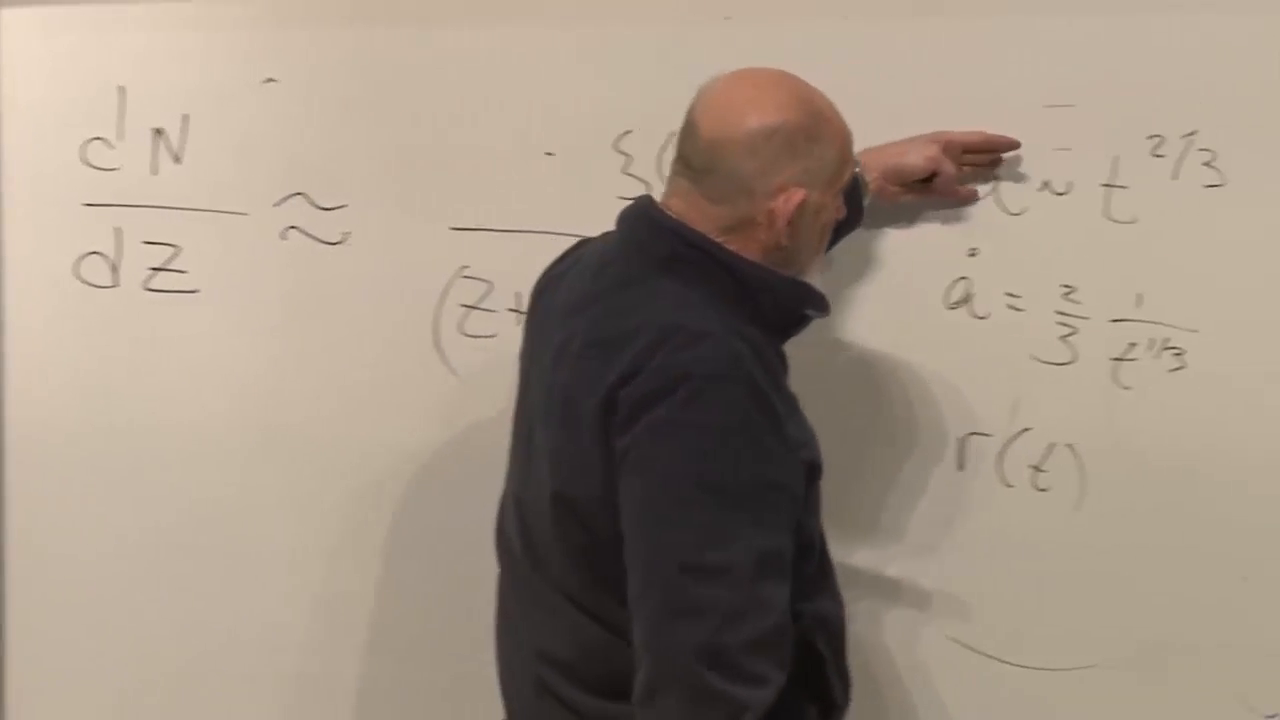
\includegraphics[width=0.84\textwidth]{lecture_06_figure_05.png}
\caption{Tafelbild mit der Beziehung zwischen \(dN/dz\) und den Modellfunktionen. Die linke Seite sowie \(a\sim t^{2/3}\), \(\dot a\) und \(r(t)\) auf der rechten Seite sind sichtbar; der Dozent verdeckt einen Teil des Nenners. Gleichung~\eqref{eq:c06-dndz} wurde unabhängig davon hergeleitet.}
\label{fig:c06-dndz-board}
\lectureframe{01:22:24.114}
\end{figure}

Es gibt nichts Weiteres auszuwerten, bis ein Modell gewählt wurde. Ein vorgegebenes \(a(t)\) bestimmt \(\dot a(t)\); Gleichung~\eqref{eq:c06-null-ray} bestimmt \(r(t)\), und Gleichung~\eqref{eq:c06-redshift} ermöglicht es, jede Größe durch \(z\) auszudrücken. Unterschiedliche Zustandsgleichungen ergeben unterschiedliche Funktionen \(dN/dz\) und \(F(z)\). Genau dadurch können die Beobachtungen zwischen Modellen unterscheiden.

\section{Von Testparametern zum besten Fit}

Das Vorgehen ist direkt:
\begin{equation}
(\Omega_r,\Omega_m,\Omega_\Lambda,\Omega_k)
\longrightarrow
a(t)
\longrightarrow
\left\{F(z),\frac{dN}{dz}\right\}.
\label{eq:c06-fit-pipeline}
\end{equation}
Man wählt heutige Parameter, löst die Friedmann-Gleichung, verfolgt radiales Licht, berechnet Helligkeit und Quellenzahlen in Abhängigkeit von der Rotverschiebung und vergleicht die Kurven mit den Daten. Ein schlechter Vergleich verwirft den Parametersatz. Zusammen schränken die beiden Observablen sowohl den Expansionsverlauf als auch die räumliche Geometrie ein.

\begin{figure}[htbp]
\centering
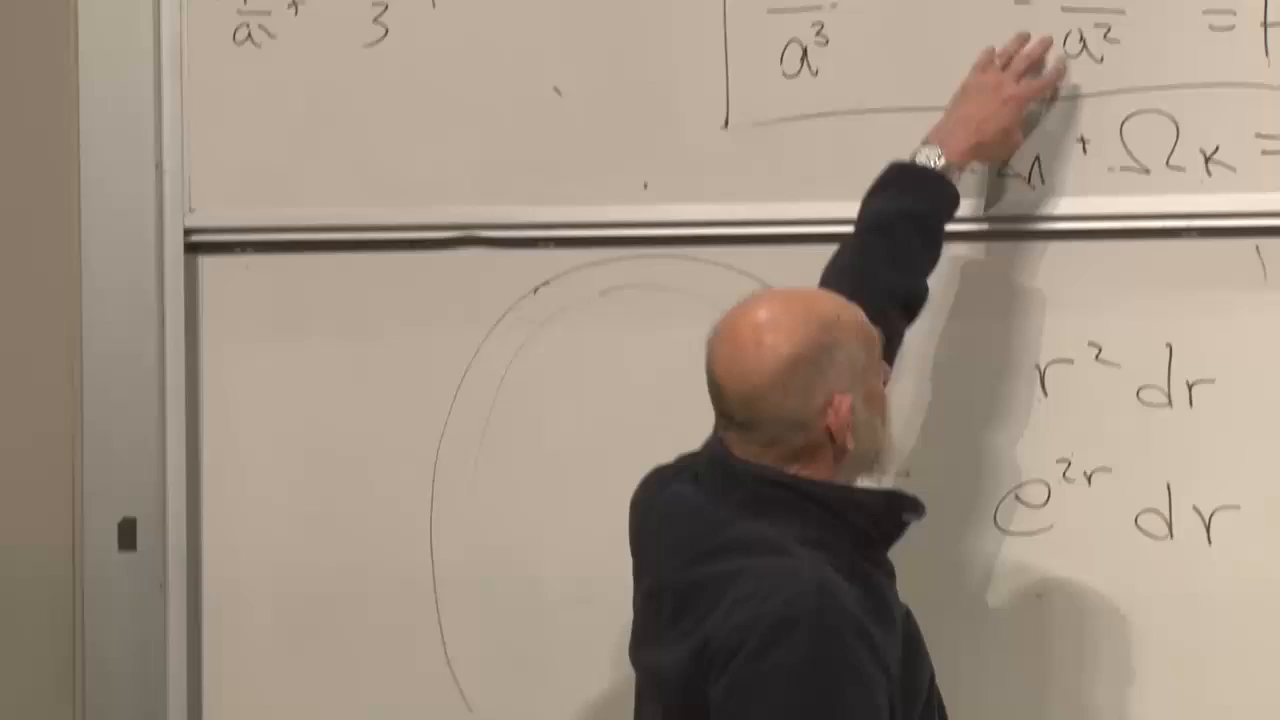
\includegraphics[width=0.84\textwidth]{lecture_06_figure_06.png}
\caption{Das alte Modell aus Materie und Krümmung an der oberen Tafel sowie die Faktoren für flache und hyperbolische Schalen \(r^2dr\) und \(e^{2r}dr\) an der unteren Tafel. Teile der Friedmann-Gleichung sind verdeckt; das Bild dient daher als ergänzender Beleg, nicht als Quelle einer Gleichung.}
\label{fig:c06-old-model-board}
\lectureframe{01:24:27.863}
\end{figure}

Das alte Modell,
\begin{equation}
H^2=\frac{C_m}{a^3}-\frac{k}{a^2},
\qquad k=-1,
\end{equation}
scheitert sowohl am Zusammenhang zwischen Helligkeit und Rotverschiebung als auch an der Prüfung anhand der Quellenzahlen. Supernovae sind im relevanten Rotverschiebungsbereich die nützlichsten Standardkerzen. Der in der Vorlesung erfolgreiche Parametersatz lautet
\begin{equation}
\boxed{
\Omega_r\simeq0,\qquad
\Omega_m\simeq0.3,\qquad
\Omega_\Lambda\simeq0.7,\qquad
\Omega_k\simeq0
}.
\label{eq:c06-best-fit}
\end{equation}
Die Materie umfasst hier sowohl leuchtende als auch Dunkle Materie. Diese Werte geben den Fit aus der Zeit der Vorlesung wieder; die bleibende Erkenntnis ist die Anpassungsmethode und die Notwendigkeit einer dominierenden, sich nicht verdünnenden Komponente, nicht die letzte angegebene Dezimalstelle.

\subsection{Fragen zu Messgrößen und Fitparametern}

\begin{classroomqa}
\audiencequestion{Wurde \(\Lambda\) bereits vorausgesetzt, als das alte Modell eines offenen Universums besprochen wurde?}
\lecturerresponse{Nein. Im ersten Teil wurde bewusst das ältere Modell mit \(\Lambda=0\) rekonstruiert. Die Werte in Gleichung~\eqref{eq:c06-best-fit} beschreiben den späteren modernen Fit. Das alte Modell wurde nicht stillschweigend abgeändert, sondern anhand von \(F(z)\) und \(dN/dz\) geprüft und verworfen. \lecturetimestamp{01:26:45--01:27:07}}
\end{classroomqa}

\begin{classroomqa}
\audiencequestion{Wie wird \(\Omega_\Lambda\) bestimmt, wenn sich Vakuumenergie nicht wie lokale Materie direkt messen lässt?}
\lecturerresponse{Man beginnt mit probeweise gewählten Parametersätzen. Jeder Satz legt eine Friedmann-Lösung und damit vorhergesagte Funktionen \(F(z)\) und \(dN/dz\) fest. Diese Vorhersagen werden mit den Beobachtungen verglichen; schlechte Fits werden verworfen, und der beste Parameterbereich bleibt übrig. Die Zahl \(0.7\) ist eine aus dem Fit abgeleitete Größe und kein unmittelbarer Messwert eines Vakuumenergie-Messgeräts. \lecturetimestamp{01:27:08--01:29:59; 01:31:57--01:33:40}}
\end{classroomqa}

\begin{classroomqa}
\audiencequestion{Woher stammt der heutige Skalenfaktor \(a_0\)?}
\lecturerresponse{Die Normierung von \(a\) ist teilweise Konvention. Ein vollständiges, an \(H_0\) gebundenes Modell liefert jedoch die heutige physikalische Krümmungsskala, sofern \(k\ne0\). Sobald das Modell die Rotverschiebungsbeobachtungen beschreibt, bestimmt seine Funktion \(a(t)\) den heutigen Zeitpunkt und die zugehörige Skala. \lecturetimestamp{01:29:59--01:30:42}}
\end{classroomqa}

\begin{classroomqa}
\audiencequestion{Verfälscht der Blick Milliarden Jahre zurück eine Anpassung, die auf den heutigen Parametern beruht?}
\lecturerresponse{Der Blick in die Vergangenheit ist keine Verfälschung, sondern das Signal. Die heutigen Parameter werden in die Friedmann-Gleichung eingesetzt, die daraus eine vollständige Entwicklung von \(a(t)\) ergibt. Der vorhergesagte Lichtkegel berücksichtigt bereits, dass Materie bei kleineren Werten von \(a\) stärker ins Gewicht fiel und in hinreichend großer Entfernung in die Vergangenheit die Strahlung dominiert. Ein Modell, das diese Entwicklung ignorierte, würde die Daten nicht beschreiben. \lecturetimestamp{01:30:43--01:31:55}}
\end{classroomqa}

\begin{classroomqa}
\audiencequestion{Welche heutigen Größen werden vergleichsweise direkt gemessen?}
\lecturerresponse{Die Strahlungsdichte wird gemessen und ist heute vernachlässigbar. Die Hubble-Rate wird anhand der Entfernungs-Rotverschiebungs-Beziehung gemessen. Die Gesamtdichte der Materie wird aus ihrer Gravitationswirkung erschlossen; sie umfasst sichtbare und dunkle Materie. Teilt man sie durch die kritische Skala \(3H_0^2/(8\pi G)\), erhält man \(\Omega_m\). Der verbleibende Spielraum zu späten Zeiten betrifft vor allem die Vakuumenergie und die Krümmung. \lecturetimestamp{01:33:40--01:35:32}}
\end{classroomqa}

\begin{classroomqa}
\audiencequestion{Wenn sowohl \(\Omega_\Lambda\) als auch \(\Omega_k\) unbekannt sind, warum gibt es nach Festlegung von \(\Omega_m\) nur einen unabhängigen freien Parameter für die späte Entwicklung?}
\lecturerresponse{Weil Gleichung~\eqref{eq:c06-sum-rule} eine Bedingung vorgibt. Wenn \(\Omega_r\) vernachlässigbar und \(\Omega_m\) gemessen ist, legt die Wahl eines Probewerts für \(\Omega_\Lambda\) den verbleibenden Wert \(\Omega_k=1-\Omega_m-\Omega_\Lambda\) fest. Dieselbe eindimensionale Familie lässt sich ebenso durch die Krümmung parametrisieren. Beispielsweise ist \(\Omega_\Lambda=0.4\) zusammen mit \(\Omega_k=0.3\) eine zulässige Wahl, wenn \(\Omega_m=0.3\); verworfen wird sie nur, weil ihre vorhergesagten Kurven schlecht zu den Daten passen, nicht weil die Summenregel sie ausschließt. \lecturetimestamp{01:35:33--01:39:09}}
\end{classroomqa}

\begin{classroomqa}
\audiencequestion{Wie kann \(k\) nur die Werte \(+1,0,-1\) annehmen, während \(\Omega_k\) stetig variiert, und stimmen die Dimensionen?}
\lecturerresponse{Das diskrete \(k\) gibt nur das Vorzeichen und die normierte Geometrie an. Der stetige Krümmungsradius wird durch \(a_0\) bestimmt, sodass \(-k/(a_0^2H_0^2)\) ein Kontinuum von Werten annehmen kann. In Einheiten mit \(c=1\) haben inverse Länge und inverse Zeit dieselbe Dimension; stellt man die üblichen Einheiten wieder her, erhält man die erforderlichen Potenzen von \(c\). \lecturetimestamp{01:39:10--01:40:07}}
\end{classroomqa}

\begin{classroomqa}
\audiencequestion{Setzt die Zählmethode Homogenität und Isotropie voraus, obwohl sich Galaxienpopulationen entwickeln?}
\lecturerresponse{Sie setzt räumliche Homogenität und Isotropie auf hinreichend großen räumlichen Schnitten voraus. Diese Symmetrien lassen sich prüfen, indem man verschiedene Richtungen bei gleicher Rotverschiebung vergleicht. Die Entwicklung der Quellen ist eine davon getrennte Frage: Populationen aus verschiedenen Epochen müssen nicht identisch sein. Daher berücksichtigen praktische Analysen Auswahlwirkungen und Entwicklung, statt eine zeitlich unveränderliche Zahlendichte zu unterstellen. Die einfache Herleitung isoliert zunächst den geometrischen Faktor; diese Verfeinerungen kommen später hinzu. \lecturetimestamp{01:40:08--01:41:08}}
\end{classroomqa}

\section{Die Dichteanteile entwickeln sich}

Gleichung~\eqref{eq:c06-budget} gilt zu jedem Zeitpunkt, aber die \(\Omega\) in Gleichung~\eqref{eq:c06-omegas} sind für den heutigen Zeitpunkt definiert. Ihre zeitabhängigen Entsprechungen ändern sich, weil die vier Terme mit unterschiedlichen Potenzen von \(a\) skalieren. In ferner Vergangenheit gilt
\begin{equation}
\Omega_r(t)\longrightarrow1.
\end{equation}
Da die Strahlung schneller verdünnt wird, wächst der Materieanteil und nähert sich der Dominanz. Später verdünnt sich auch die Materie, während \(\Lambda\) konstant bleibt. In ferner Zukunft gilt daher
\begin{equation}
\Omega_\Lambda(t)\longrightarrow1.
\end{equation}
Der Materieanteil ist anfangs also klein, nähert sich während der Materieära dem Wert eins und nimmt wieder ab, sobald die Vakuumenergie die Dominanz übernimmt. Auch die Krümmung wird, falls sie von null verschieden ist, schließlich gegenüber einer positiven konstanten \(\Lambda\) vernachlässigbar.

\begin{classroomqa}
\audiencequestion{Bedeutet ein kleiner heutiger Krümmungsanteil, dass das Universum bei seiner Expansion immer flacher wird?}
\lecturerresponse{Die physikalische Krümmungsskala wächst mit \(a\), und relativ zu einer positiven kosmologischen Konstante wird der Krümmungsbeitrag \(a^{-2}\) immer weniger wichtig. Das ist mit der Formulierung \emph{groß ist flach} gemeint. Das diskrete Topologieetikett \(k\) ändert sich dadurch nicht; gemeint ist, dass die lokale Krümmung und die relative dynamische Bedeutung der Krümmung abnehmen. \lecturetimestamp{01:47:13--01:47:42}}
\end{classroomqa}

\begin{classroomqa}
\audiencequestion{Zeigte das angepasste Modell unerklärte systematische Abweichungen, und wie genau war die Aussage?}
\lecturerresponse{In der Vorlesung werden auf diesem Genauigkeitsniveau keine bekannten systematischen Fehler des Rahmens berichtet; die Kosmologie wird als Präzisionskosmologie mit einer Genauigkeit von ungefähr einem Prozent beschrieben, nicht von einem Zehntel oder Hundertstel Prozent. Diese Aussage ist historisch und darf nicht als zeitlos gültige aktuelle Fehlerangabe verstanden werden. \lecturetimestamp{01:45:40--01:46:19}}
\end{classroomqa}

\begin{classroomqa}
\audiencequestion{Lässt sich die räumliche Krümmung durch direkte Triangulation prüfen, statt nur anhand der Helligkeit von Supernovae und von Zählungen?}
\lecturerresponse{Ja. Das Winkelspektrum der kosmischen Mikrowellenhintergrundstrahlung liefert eine physikalische Standardskala und damit ein großes kosmisches Dreieck. Supernova-Daten allein lieferten nicht die vollständige Krümmungsaussage der Vorlesung mit Prozentgenauigkeit; durch die Kombination mit der Geometrie des Mikrowellenhintergrunds ließ sich die Prüfung präzisieren. Darum geht es in der nächsten Vorlesung. \lecturetimestamp{01:46:19--01:47:12}}
\end{classroomqa}

\section{Was bleibt}

Die zentrale Erkenntnis ist keine Liste aus vier Zahlen, sondern eine Methode. Ein Satz kosmologischer Parameter ergibt \(a(t)\); die Metrik sagt dann voraus, wie sich Licht ausbreitet, wie hell Quellen erscheinen und wie viele Quellen beobachtet werden. Die Übereinstimmung prüft sowohl die gewählten Parameter als auch den Friedmann-Rahmen, der sie miteinander verknüpft. Es gibt keinen Grund anzunehmen, dass ein beliebiger Parametersatz zu den Daten passt.

Das ältere Modell mit sichtbarer Materie und negativer Krümmung scheiterte. Dunkle Materie ergänzte den gravitativen Materiebestand, schloss für sich genommen aber nicht die alte Friedmann-Bilanz. Die erfolgreiche Anpassung zur Zeit der Vorlesung erforderte näherungsweise
\begin{equation}
\Omega_m\simeq0.3,
\qquad
\Omega_\Lambda\simeq0.7,
\qquad
\Omega_k\simeq0,
\end{equation}
Für die Genauigkeit der Krümmungsbestimmung war der Mikrowellenhintergrund von wesentlicher Bedeutung. Das Modell ist glaubwürdig, weil mehrere unabhängige Beobachtungen durch eine gemeinsame dynamische Theorie beschrieben werden und sich im selben Parameterbereich vereinbaren lassen.
